\section{Implementering af DSP modul}\label{sec:implementering_dsp}
DSP modulet har til opgave at beregne koefficienter, beregne amplitude (til lcd'en), udføre det 
digitale filter på de samples der modtages mm.. 
Modulet består af \textit{dsp.c}, \textit{dsp.h} som kan findes i kildekoden. 


\begin{figure}[ht]
\centering
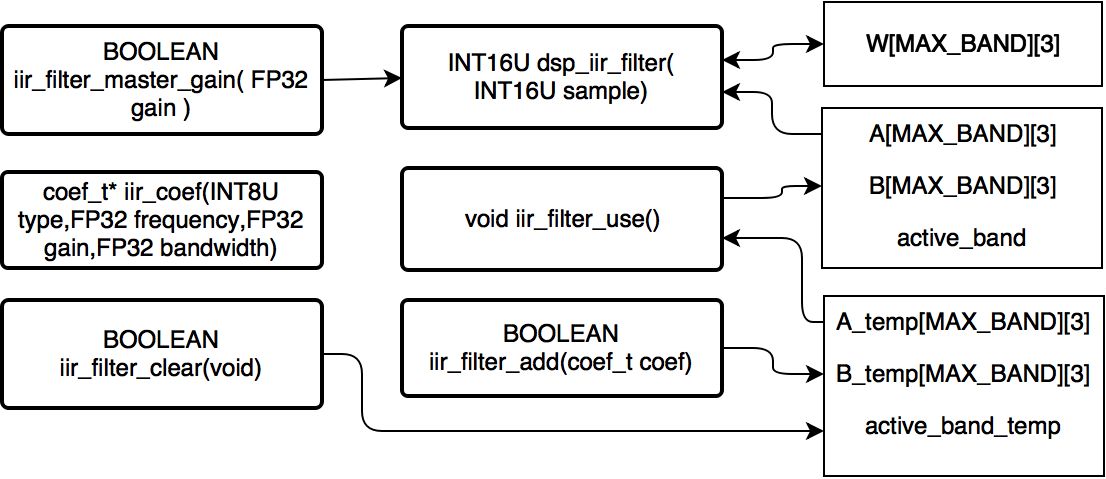
\includegraphics[scale = 0.3]{billeder/finalflow_dsp}
\caption{Blokdiagram der illustrerer dataflowet.}
\label{fig:data_flow_imp}
 \end{figure}


\subsection{API oversigt}
De funktionaliteter DSP modulet stiller til rådighed er følgende:

\texttt{INT16U dsp\_iir\_filter( INT16U sample);}\\
Filtrerer et givent sample med de koefficienter der er gemt i matricerne \texttt{A[][]},\texttt{B[][]}.\\

\texttt{BOOLEAN iir\_filter\_master\_gain( FP32 gain ); }\\
Omregner \texttt{gain} fra $dB$ og sætter master\_gain. Returnerer false hvis \texttt{gain} overskrider $\pm 20dB$.\\

\texttt{coef\_t* iir\_coef(INT8U type,FP32 frequency,FP32 gain,FP32 bandwidth);}\\
Beregner et 2. ordens filters koefficienter ud fra en filter type og de givne parametre hvorefter koefficienterne returneres i \texttt{coef\_t} struktur'en.\\

\texttt{BOOLEAN iir\_filter\_add(coef\_t coef);}\\
Tilføjer koefficienter for et 2. ordens filter til \texttt{A\_temp[][]}, \texttt{B\_[][]}. Returnerer false hvis der tilføjes mere end 10 bånd.\\

\texttt{void iir\_filter\_use();} \\
Tager de koefficienter der er tilføjet og overfører dem over til \texttt{A[][]}, \texttt{B[][]} hvorefter at equalizeren bliver slået til.\\

\texttt{BOOLEAN iir\_filter\_clear(void);} \\ 
Nulstiller de midlertidige koefficienter \texttt{A\_temp[][]}, \texttt{B\_temp[][]} og antal aktive bånd. \\

\texttt{void dsp\_filter\_log\_freq( INT16U* frequency\_arr,INT8U size );} \\ 
Beregner en logaritmisk inddelt frekvens array på \texttt{size} elementer. \\

\texttt{FP32 dsp\_filter\_amplitude( INT16U frequency );}\\
Beregner amplituden af den aktive equalizer ved en given frekvens. Returnerer resultatet i $dB$. \\

Data structur til at holde koefficienterne:\\
\lstset{language=C,
	frame=sigle,
	basicstyle=\ttfamily\small,
	emph={FP32},
	emphstyle={\color{blue}},
	keepspaces=true,%
	%frame=single,
%	numbers=left,
%	numbersep=5pt,
	numberstyle=\tiny\color{black},
	keywordstyle=\color{red}\ttfamily,
	stringstyle=\color{blue}\ttfamily,
	commentstyle=\color{OliveGreen}\ttfamily,
	morecomment=[l][\color{magenta}]{\#}
}
\begin{tabular}{l}
\begin{lstlisting}
typedef struct coef{
  FP32 a[3];      // a coefficients of a biquad
  FP32 b[3];      // b coefficients of a biquad 
}coef_t;
\end{lstlisting}
\end{tabular}




\section{Delkonklusion}

\note{
	Test af CPU og hvordan det er at implementere
}





